% Options for packages loaded elsewhere
\PassOptionsToPackage{unicode}{hyperref}
\PassOptionsToPackage{hyphens}{url}
%
\documentclass[
]{article}
\usepackage{lmodern}
\usepackage{amssymb,amsmath}
\usepackage{ifxetex,ifluatex}
\usepackage{minted}
\ifnum 0\ifxetex 1\fi\ifluatex 1\fi=0 % if pdftex
  \usepackage[T1]{fontenc}
  \usepackage[utf8]{inputenc}
  \usepackage{textcomp} % provide euro and other symbols
\else % if luatex or xetex
  \usepackage{unicode-math}
  \defaultfontfeatures{Scale=MatchLowercase}
  \defaultfontfeatures[\rmfamily]{Ligatures=TeX,Scale=1}
\fi
% Use upquote if available, for straight quotes in verbatim environments
\IfFileExists{upquote.sty}{\usepackage{upquote}}{}
\IfFileExists{microtype.sty}{% use microtype if available
  \usepackage[]{microtype}
  \UseMicrotypeSet[protrusion]{basicmath} % disable protrusion for tt fonts
}{}
\makeatletter
\@ifundefined{KOMAClassName}{% if non-KOMA class
  \IfFileExists{parskip.sty}{%
    \usepackage{parskip}
  }{% else
    \setlength{\parindent}{0pt}
    \setlength{\parskip}{6pt plus 2pt minus 1pt}}
}{% if KOMA class
  \KOMAoptions{parskip=half}}
\makeatother
\usepackage{xcolor}
\IfFileExists{xurl.sty}{\usepackage{xurl}}{} % add URL line breaks if available
\IfFileExists{bookmark.sty}{\usepackage{bookmark}}{\usepackage{hyperref}}
\hypersetup{
  hidelinks,
  pdfcreator={LaTeX via pandoc}}
\urlstyle{same} % disable monospaced font for URLs
\usepackage{graphicx,grffile}
\makeatletter
\def\maxwidth{\ifdim\Gin@nat@width>\linewidth\linewidth\else\Gin@nat@width\fi}
\def\maxheight{\ifdim\Gin@nat@height>\textheight\textheight\else\Gin@nat@height\fi}
\makeatother
% Scale images if necessary, so that they will not overflow the page
% margins by default, and it is still possible to overwrite the defaults
% using explicit options in \includegraphics[width, height, ...]{}
\setkeys{Gin}{width=\maxwidth,height=\maxheight,keepaspectratio}
% Set default figure placement to htbp
\makeatletter
\def\fps@figure{htbp}
\makeatother
\setlength{\emergencystretch}{3em} % prevent overfull lines
\providecommand{\tightlist}{%
  \setlength{\itemsep}{0pt}\setlength{\parskip}{0pt}}
\setcounter{secnumdepth}{-\maxdimen} % remove section numbering

\date{}

\pagenumbering{gobble}
\begin{document}

\begin{figure}
\centering

\includegraphics{icpc.jpg}
\end{figure}

\hypertarget{header-n33}{%
\begin{center}
\section{Monash Collegiate Programming Contest }\label{header-n33}
\end{center}
}

\hypertarget{header-n37}{%
\centering
\subsection{ \texorpdfstring{Practice Round}{Practice Round} }}

\hypertarget{header-n37}{%
\centering
\subsection{ \texorpdfstring{24th, August, 2019}{ 24th, August, 2019} }}

\begin{center}\rule{0.5\linewidth}{\linethickness}\end{center}

\newpage

\hypertarget{header-n43}{%
\section{FQAs}\label{header-n43}}

\begin{quote}
Q: Why I passed all samples, but still get \texttt{Wrong\ Answer\ (WA)} ?
\end{quote}

\begin{itemize}
\item
  There are multiple secret test cases, failing on any of them causes
  \texttt{Wrong\ Answer}, so you'll have to spot the bug by yourself.
\end{itemize}


\begin{quote}
Q: What is \texttt{Time\ Limit\ Exceeded\ (TLE)} ?
\end{quote}

\begin{itemize}
\item
  Your program runs out of time limit; this error doesn't allow you to
  know if your program would reach the correct solution to the problem
  or not.
\end{itemize}


\begin{quote}
  Q: What is \texttt{Memory\ Limit\ Exceeded\ (MLE)} ?
\end{quote}

\begin{itemize}
\item
  Your program tried to use more memory than the judge allows. 
\end{itemize}

\begin{quote}
  Q: What is \texttt{Runtime\ Error\ (RE)}
\end{quote}

\begin{itemize}
\item
  Your program failed during the execution (segmentation fault, floating
  point exception...). The exact cause is not reported to the user to
  avoid hacking. 
\end{itemize}

\begin{quote}
  Q: There are \texttt{Input\ file:\ standard\ input},
\texttt{Output\ file:\ standard\ output} in my problem statement, what
do these mean? Do I need to create files?
\end{quote}

\begin{itemize}
\item
  Reading from standard input (\texttt{stdin}) means reading data which
  you are typing on your keyboard, and outputting to standard output
  (\texttt{stdout}) means printing data to your console. So it's not
  necessary to create files.
\end{itemize}

\begin{quote}
  Q: How to read and request clarifications?
\end{quote}

\begin{itemize}
\item
  \begin{figure}
  \centering
  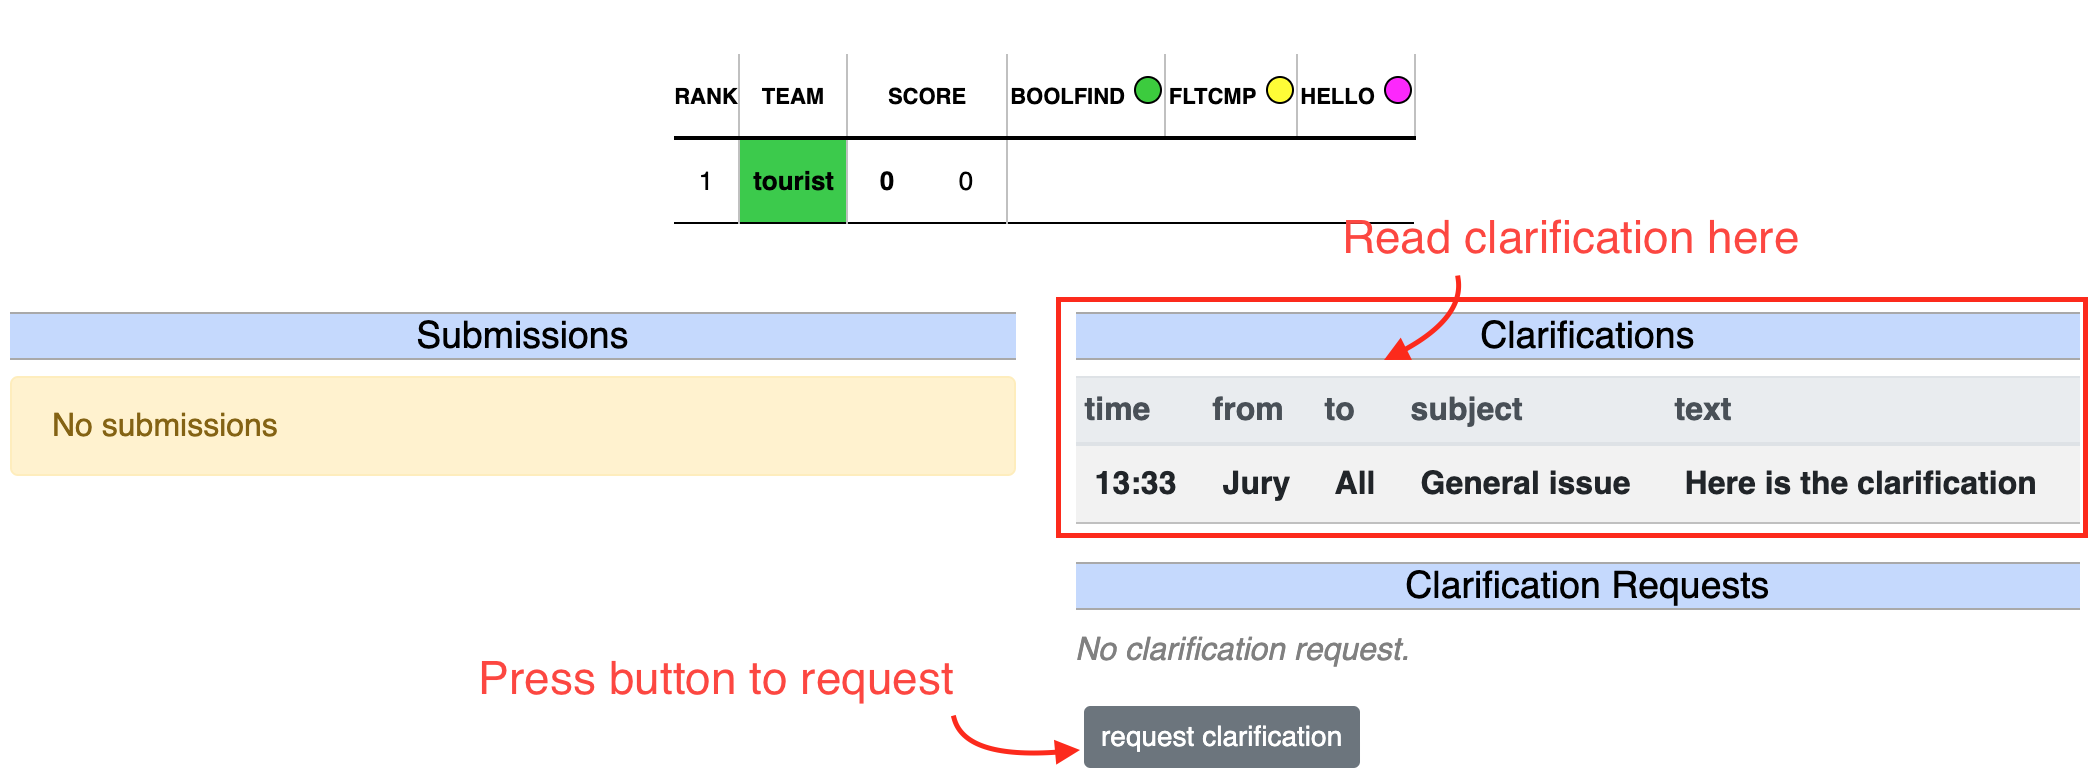
\includegraphics{clarification.png}
  \end{figure}
\end{itemize}

\begin{center}\rule{0.5\linewidth}{\linethickness}\end{center}

\hypertarget{header-n119}{%
\section{Tips}\label{header-n119}}

\begin{itemize}
\item
  Pay attention to \texttt{Time\ limit}, \texttt{Memory\ limit}
  constraints in your problem statement when you get
  \texttt{Time\ Limit\ Exceeded} or \texttt{Memory\ Limit\ Exceeded}
  verdict.
\item
  \texttt{C++} can nearly run \( 10^8\) basic operations (e.g.
  \texttt{+,-}) in 1 second, \texttt{Python} can nearly run \(10^6\)
  basic operations in 1 second, and you can esitmate your program
  running time based on these info and your compexity analysis to avoid
  \texttt{Time\ Limit\ Exceeded}.

\item Instead of typing on keyboard, a more convenient way for local testing in command line is:

\begin{minted}[frame=lines, bgcolor=lightgray,fontsize=\footnotesize]{bash}
./myprogram < sample.in > myoutput
diff myoutput sample.out
\end{minted}
    where \texttt{<} is redirect all contents of file \texttt{sample.in} to \texttt{standard input}, and \texttt{>} is redirect your \texttt{standard output} to the file \texttt{myoutput},
    and \texttt{diff} is to check the difference between your output and the expected answer.
\end{itemize}

\item
  \huge Good Luck \& Have Fun!

\begin{center}\rule{0.5\linewidth}{\linethickness}\end{center}
\end{document}
